Come affermato nella~\cref{subsec:overlapping}, il clustering partizionante ignora le singolarità delle traiettorie.
Per superare il problema descritto sopra, gli algoritmi di clustering sovrapposto effettuano una divisione di ogni traiettoria
in sotto-traiettorie e effettuano un clustering partizionante su queste sotto-traiettorie.

Una famiglia di algoritmi basati su questa idea è \textit{Partition and group based algorithm}.
Il focus principale di questa categoria è l'individuazione dei segmenti e
dei punti in cui ``spezzare'' la traiettoria originale.
Per risolvere questo problema sono state ipotizzate diverse soluzioni,
ad esempio il framework \textit{DSC} (Distribuited Subtrajectory Clustering)~\cite{tampakis2019scalable} utilizza una metrica basata
sul cambio di densità nell'intorno dei punti della traiettoria per determinare le divisioni.
In una prima fase DSC compie una operazione di \textit{self-join} su ogni traiettoria, ricercando tutte le traiettorie aventi uno spaziotempo comune di almeno \(k\) istanti con ogni singolo elemento del dataset.
Questa misura viene effettuata tramite LCSS.
Successivamente vengono determinati i punti di separazione di ogni traiettoria: ciò viene fatto analizzando il vicinato creato nella fase precedente e separando la traiettoria ogni volta che la densità o la composizione di quest'ultimo cambia in maniera significativa.
Infine vengono i segmenti così originati sono sottoposti a una versione modificata di k-means: sono individuati \(R\) rappresentati nel dataset e ogni segmento viene attribuito ad un unico rappresentante.
Alla fine di questo passo i cluster vengono raffinati così da eliminare segmenti ripetuti e fondere cluster simili.
La~\cref{fig:chap-1:dsc} mostra un esempio di clustering effettuato da DSC: com'è possibile vedere
ogni traiettoria viene divisa in più segmenti ed è assegnata a diversi cluster.

\begin{figure}
\centering
  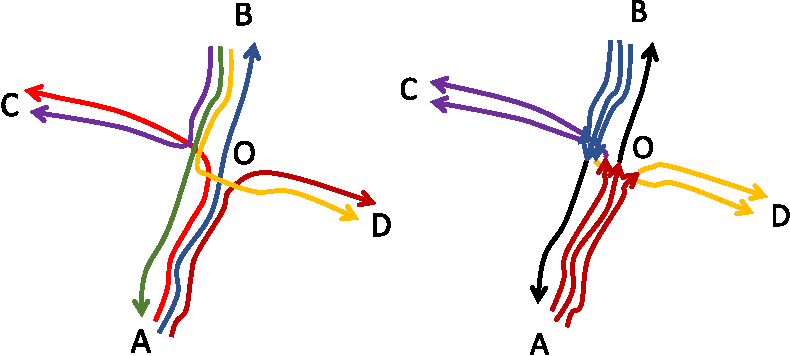
\includegraphics[scale=.8]{res/fig/sec-1/DSCDataset.pdf}
  \caption{Traiettorie di partenza (a sinistra), Cluster individuati da DSC (a destra), Fonte:~\cite{tampakis2019scalable} }%
  \label{fig:chap-1:dsc}
\end{figure}    


Il clustering sovrapposto permette di conservare le relazioni intra-cluster, tuttavia una frammentazione troppo fine può causare
la perdita di \textit{rare pattern}, ad esempio eventi significanti che accadono con una bassa frequenza~\cite{DBLP:journals/tkdd/KohR16, DBLP:journals/geoinformatica/HuangPX06}.